\documentclass{beamer}
\usepackage{ctex, hyperref}
\usepackage[T1]{fontenc}

% other packages
\usepackage{latexsym,amsmath,xcolor,multicol,booktabs,calligra}
\usepackage{graphicx,pstricks,listings,stackengine}
\usepackage{subfigure}

\author[郝淼]{郝淼\\{指导老师:张福新}}
\title{Xenomai的LoongArch平台移植与性能优化}
\subtitle{本科毕业论文答辩}
\institute{中国科学院大学计算机科学与技术学院}
\date{2023年5月25日}
\usepackage{UCAS}

% defs
\def\cmd#1{\texttt{\color{red}\footnotesize $\backslash$#1}}
\def\env#1{\texttt{\color{blue}\footnotesize #1}}
\definecolor{deepblue}{rgb}{0,0,0.5}
\definecolor{deepred}{rgb}{0.6,0,0}
\definecolor{deepgreen}{rgb}{0,0.5,0}
\definecolor{halfgray}{gray}{0.55}

\lstset{
    basicstyle=\ttfamily\small,
    keywordstyle=\bfseries\color{deepblue},
    emphstyle=\ttfamily\color{deepred},    % Custom highlighting style
    stringstyle=\color{deepgreen},
    numbers=left,
    numberstyle=\small\color{halfgray},
    rulesepcolor=\color{red!20!green!20!blue!20},
    frame=shadowbox,
}


\begin{document}

\heiti
\begin{frame}
    \titlepage
    \begin{figure}[htpb]
        \begin{center}
            
\includegraphics[width=0.2\linewidth]{pic/CAS_Logo.png}
        \end{center}
    \end{figure}
\end{frame}

\begin{frame}
    \tableofcontents[sectionstyle=show,subsectionstyle=show/shaded/hide,subsubsectionstyle=show/shaded/hide]
\end{frame}

\section{选题背景及意义}

% \begin{frame}{选题背景及意义}
%     2023年消费电子产品展(CES)中的统计数据$^{\text{\cite{iotannon}}}$:
%     \begin{figure}[h]
%         \centering
%         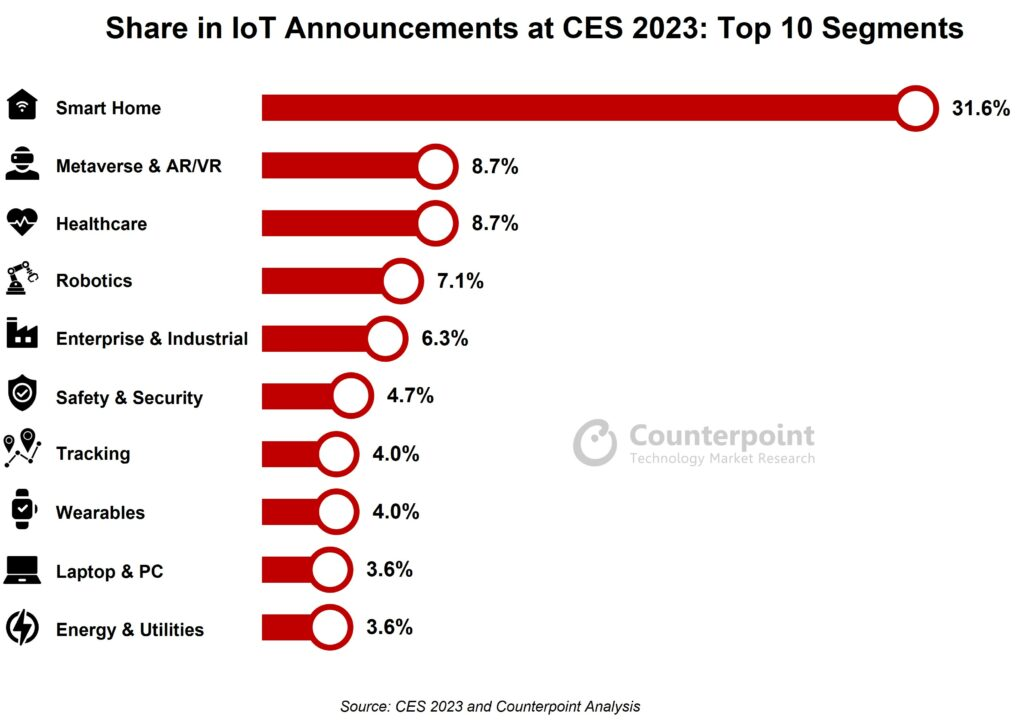
\includegraphics{img/iot-top-10.jpg}
%     \end{figure}
% \end{frame}

\begin{frame}{选题背景及意义}
    \begin{itemize}
        \item 随着\textbf{嵌入式市场}的不断繁荣,\textbf{实时操作系统}作为嵌入式平台上运行的基础软件将在未来发挥更大的作用
        \item 目前LoonArch平台支持的实时操作系统\textbf{数量较少}
        \item 基于现有成熟、易用的实时操作系统\textbf{进行LoongArch平台的移植与优化}是很有必要的
    \end{itemize}
\end{frame}

\section{研究现状}

\begin{frame}{研究现状-实时操作系统的分类}
    实时操作系统要求\textbf{外部事件}发生时,对应的\textbf{实时程序}能够在\textbf{截止时间}前完成处理。
    \begin{itemize}
        \item \textbf{硬实时:}\textbf{不允许}处理时间超过截止时间
        \item \textbf{软实时:}\textbf{允许部分}处理时间超过截止时间
    \end{itemize}
\end{frame}

\begin{frame}{研究现状-实时操作系统的实现方式}
    
        \begin{figure}[h]
            \centering
            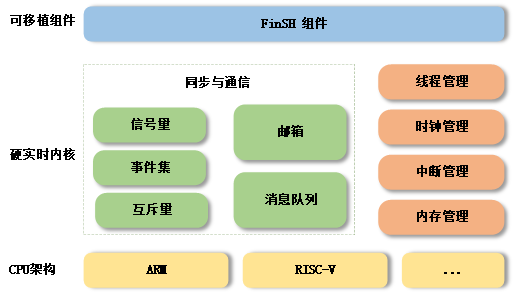
\includegraphics[height=.5\textheight]{img/rtthread.png}
        \end{figure}
    \begin{center}
        \textbf{微内核:}采用一个单独的实时内核,如RT-Thread
    \end{center}
\end{frame}

\begin{frame}{研究现状-实时操作系统的实现方式}
    
    \begin{figure}[h]
        \centering
        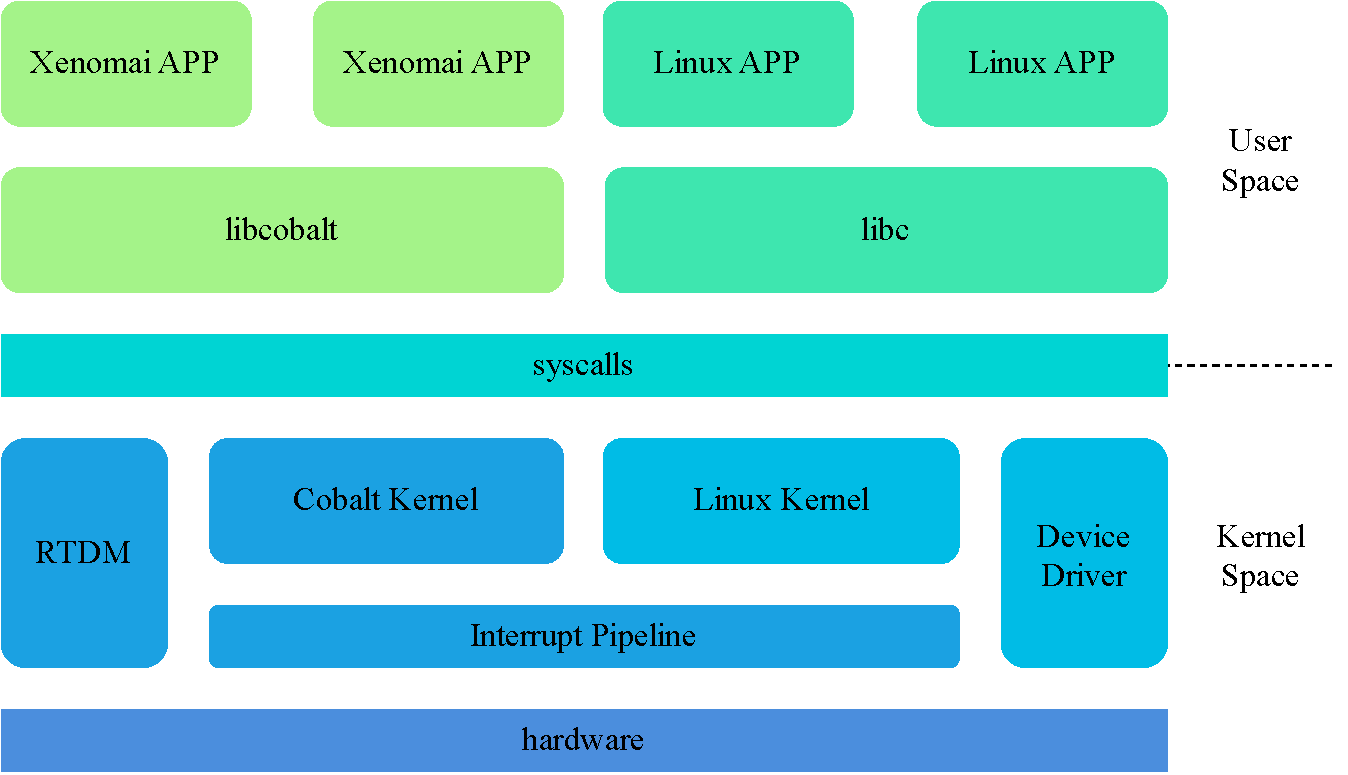
\includegraphics[height=.5\textheight]{img/Img/xenomai-prj.pdf}
    \end{figure}
    \begin{center}
        \textbf{扩展内核:}对通用内核进行修改,提升实时性,如Xenomai
    \end{center}
\end{frame}

\begin{frame}{研究现状-实时操作系统的实现方式}
    目前,LoongArch平台支持的实时操作系统包括:
    \begin{itemize}
        \item \textbf{微内核:}RT-Thread,SylixOS
        \item \textbf{扩展内核:}RTLinux
    \end{itemize}
\end{frame}

\begin{frame}{研究现状-Xenomai项目}
    \begin{minipage}{0.45\linewidth}
        % \medskip
        %\hspace{2cm}
        \begin{figure}[h]
            \centering
            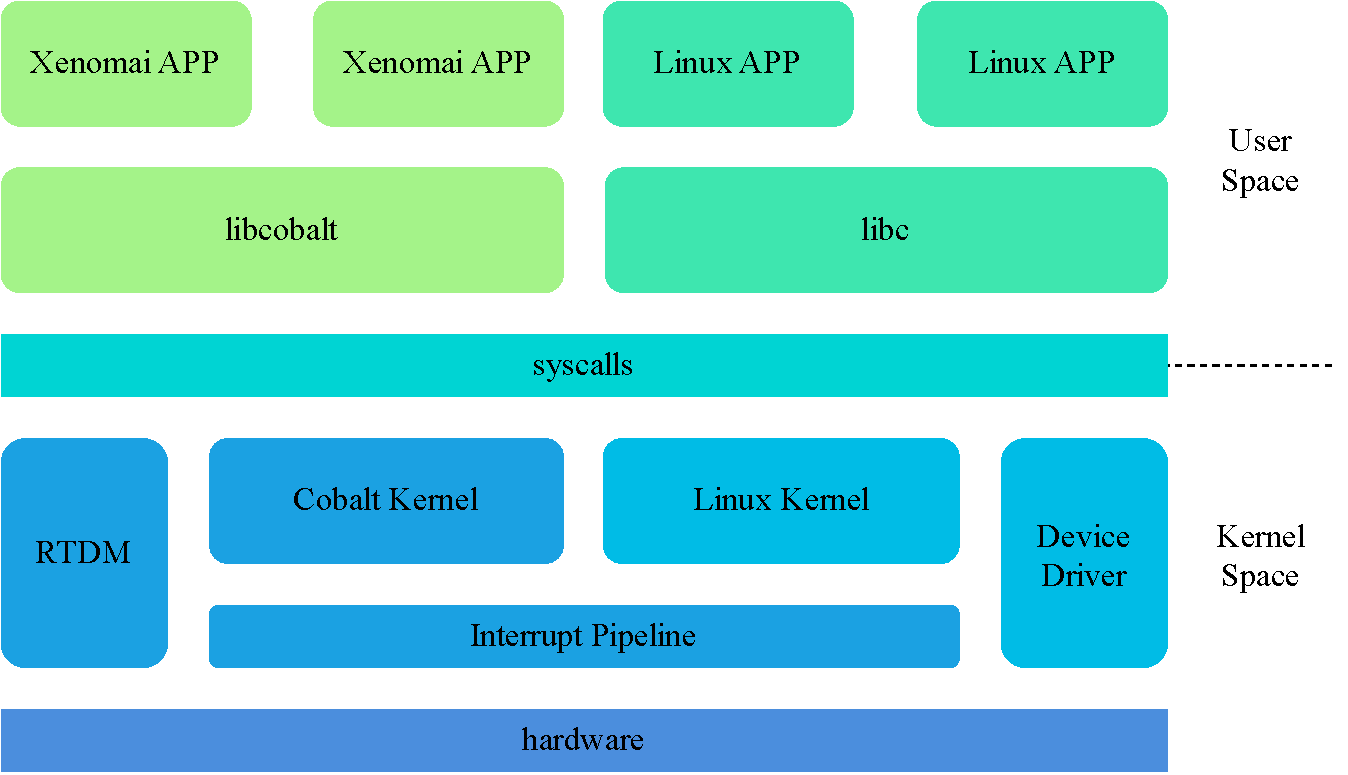
\includegraphics[height=.45\textheight]{img/Img/xenomai-prj.pdf}
        \end{figure}
    \end{minipage}\hspace{1.5cm}
    \begin{minipage}{0.35\linewidth}
        \begin{itemize}
            \item 扩展内核架构
            \item 基于ADEOS的“双内核”系统
            \item I-pipe,cobalt,libcobalt
        \end{itemize}
    \end{minipage}
    \medskip
    \begin{itemize}
        \item 实时性:Xenomai能够提供\textbf{硬实时}保障
        \item 兼容性:libcobalt实现了与\textbf{VxWorks、POSIX等兼容}的API
    \end{itemize}
\end{frame}

\section{主要研究内容}

\subsection{实时任务模型}

\begin{frame}{实时任务模型-简介}
    Hideyuki Tokuda等在1990年为了研究可预测的实时调度器,建立了实时线程模型(RT-Thread Model),但该模型缺乏对\textbf{外部事件}和\textbf{实时操作系统能力}的刻画,导致无法用于描述Xenomai中实时任务运行的模型,因此本课题基于实时线程模型建立了实时任务模型。
\end{frame}

\begin{frame}{实时任务模型-简介}
    实时任务模型可以表述为:
    \begin{equation}
        \begin{cases}
            T_i=(\Delta t_{l_i}, \Delta t_{r_i}) \\
            e_k=(C_{e_{k}}^1,C_{e_{k}}^2,C_{e_{k}}^3) \\
        \end{cases}
    \end{equation}
\end{frame}

\begin{frame}{实时任务模型-实时任务$T_i$}
    \begin{center}
        $T_i=(\Delta t_{l_i}, \Delta t_{r_i})$
    \end{center}
    \begin{figure}[h]
        \centering
        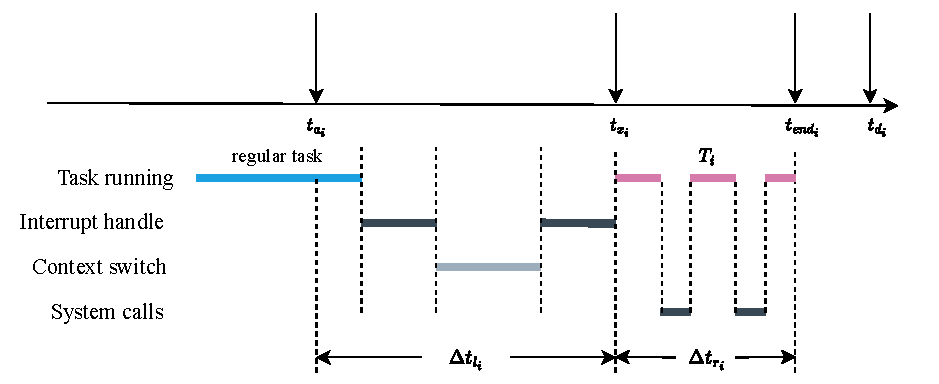
\includegraphics[height=.45\textheight]{img/Img/time-line.pdf}
    \end{figure}
    \begin{itemize}
        \item $\Delta t_{l_i} = t_{x_i}-t_{a_i}$:延迟
        \item $\Delta t_{r_i} = t_{end_i} - t_{x_i}$:运行时间
    \end{itemize}
    % \begin{minipage}{1.0\linewidth}
        % \medskip
        %\hspace{2cm}
    % \end{minipage}
    % \begin{minipage}{0.35\linewidth}
    % \end{minipage}
\end{frame}

\begin{frame}{实时任务模型-外部事件$e_k$}
    \begin{center}
        $\{T_i\}_{e_k}$为响应$e_k$的实时任务集合,$e_k=(C_{e_{k}}^1,C_{e_{k}}^2,C_{e_{k}}^3)$
    \end{center}
    \begin{figure}[h]
        \centering
        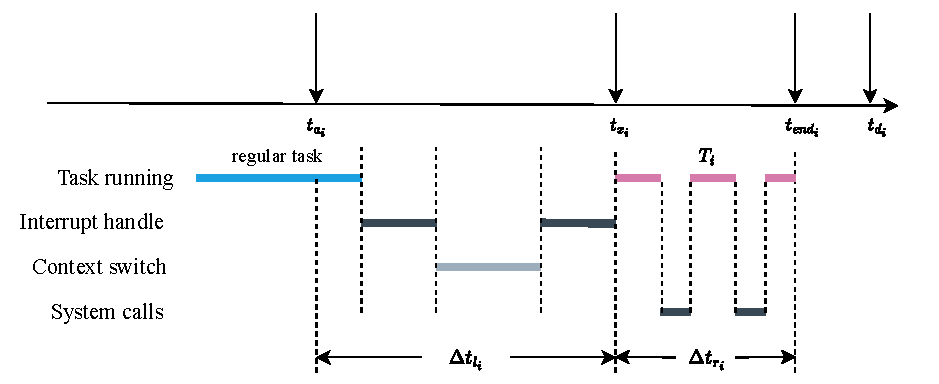
\includegraphics[height=.45\textheight]{img/Img/time-line.pdf}
    \end{figure}
    \begin{itemize}
        \item $C_{e_{k}}^1 = t_{d_i}-t_{a_i}$:刻画了外部事件的截止时间
        \item $t_{a_{i+1}}-t_{a_i}\in [C_{e_{k}}^2,C_{e_{k}}^3]$:刻画了外部事件的周期性
    \end{itemize}
\end{frame}

\begin{frame}{实时任务模型-实时约束条件}
    在实时操作系统中,希望$\{T_i\}_{e_k}$能满足约束条件
\begin{align}
    t_{end_i} \le t_{d_i} &\Leftrightarrow (t_{end_i} - t_{x_i}) + (t_{x_i} - t_{a_i}) \le t_{d_i} - t_{a_i} \\
    &\Leftrightarrow \Delta t_{r_i} + \Delta t_{l_i} \le C_{e_k}^1 \\
    &\Leftrightarrow \Delta t_{l_i} + \Delta t_{r_i} \le C_{e_k}^1\label{3}
\end{align}

当条件(\ref{3})不成立时,称系统中发生了\textbf{超时故障}
    
\end{frame}

\begin{frame}{实时任务模型-Xenomai实时原理}
    对于Xenomai而言,应尽可能缩短$\Delta t_{l_i} + \Delta t_{r_i}$:
    \begin{itemize}
        \item 使用专用的实时内核进行调度$\Rightarrow$缩短$\Delta t_{l_i}$;
        \item 实时内核提供实时系统调用$\Rightarrow$缩短$\Delta t_{r_i}$;
        \item 提供区别于普通API的实时API$\Rightarrow$帮助程序员从宏观上缩短$\Delta t_{l_i} + \Delta t_{r_i}$;
    \end{itemize}
\end{frame}
\subsection{Xenomai 的 LoongArch 平台移植}

\begin{frame}{Xenomai 的 LoongArch 平台移植}
    \begin{itemize}
        \item I-pipe:3A5000的中断结构,LoongArch Linux的中断处理过程,I-pipe的实现原理
        \item cobalt:LoongArch中的时间硬件资源,cobalt内核的工作原理,cobalt中的体系结构相关代码
        \item libcobalt:LoongArch ABI
    \end{itemize}
\end{frame}

\subsection{LoongArch Xenomai 系统的性能优化}

\begin{frame}{LoongArch Xenomai 系统的性能优化-性能评价指标}
    \begin{figure}[!htbp]
        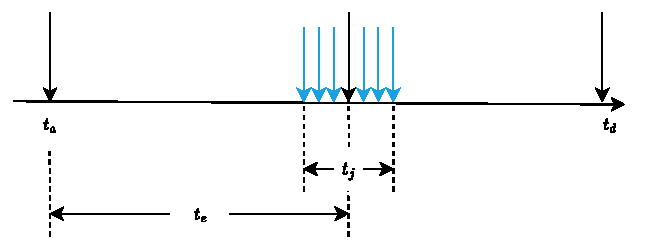
\includegraphics[width=\textwidth]{img/Img/jitter.pdf}
      \end{figure}
    \begin{itemize}
        \item 延迟期望$t_e\to$实时性
        \item 抖动$t_j\to$稳定性
        \item 硬实时约束$\to$$\max_{T_i\in\{T_i\}_{e_k}}{(\Delta t_{l_i} + \Delta t_{r_i})} \le C_{e_{k}}^1$
    \end{itemize}
\end{frame}

\begin{frame}{LoongArch Xenomai 系统的性能优化-latency测试}
    \begin{figure}[!htbp]
        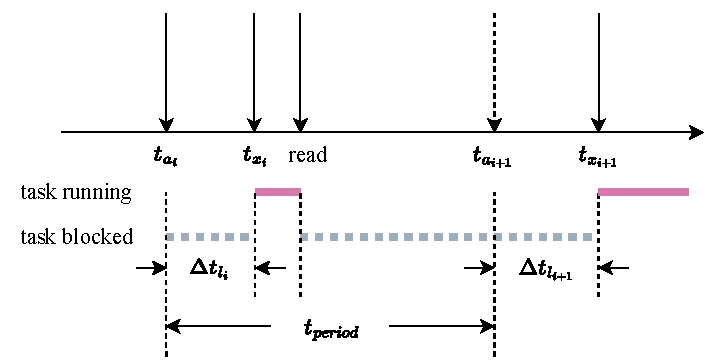
\includegraphics[width=.8\textwidth]{img/Img/latency-time-line.pdf}
    \end{figure}
    \begin{itemize}
        \item $t_j=t_{max}-t_{min}$
        \item $t_e=t_{avg}$
        \item $e_l=(t_{period}, t_{period}, t_{period})$
    \end{itemize}
\end{frame}

\begin{frame}{LoongArch Xenomai 系统的性能优化-latency测试}
    \begin{figure}[!htbp]
        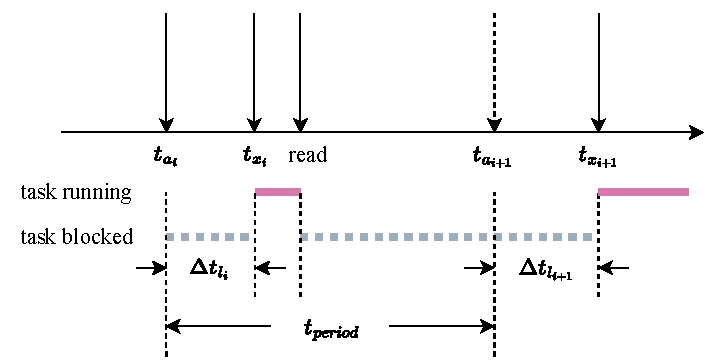
\includegraphics[width=.8\textwidth]{img/Img/latency-time-line.pdf}
    \end{figure}
    在latency测试中,$\Delta t_{r_i}\approx 0$,硬实时约束简化为$t_{max}\le t_{period}$
\end{frame}

\begin{frame}{LoongArch Xenomai 系统的性能优化-测试环境}
    \begin{itemize}
        \item latency配置:$e_l=(100\mu \text{s}, 100\mu \text{s}, 100\mu \text{s})$,硬实时约束为$t_{max}\le 100\mu \text{s}$
        \item 物理平台:
            \begin{itemize}
                \item 处理器:4核2.5GHz龙芯3A5000
                \item 桥片:龙芯7A2000
                \item 物理内存:16GB
            \end{itemize}
        \item 访存负载:{\ttfamily stress -m 4}
    \end{itemize}
\end{frame}

\begin{frame}{LoongArch Xenomai 系统的性能优化-优化方法}
    \begin{itemize}
        \item 关闭页迁移:透明巨页THP
        \item 关闭高延迟外设:声卡,实时时钟
        \item 关键路径优化:{\ttfamily xnclock\_core\_ns\_to\_ticks}与{\ttfamily xnclock\_core\_ticks\_to\_ns}
    \end{itemize}
\end{frame}

\begin{frame}{LoongArch Xenomai 系统的性能优化-对照设置}
    \begin{enumerate}
        \item 硬实时内核RTLinux,内核版本4.19
        \item 未优化Xenomai,内核版本4.19
        \item 在2.的基础上关闭页迁移
        \item 在3.的基础上关闭高延迟外设,并进行关键路径优化     
    \end{enumerate}
\end{frame}

\begin{frame}{LoongArch Xenomai 系统的性能优化-无负载测试结果}
    \begin{figure}[H]
        \centering  %图片全局居中
        \vspace{-0.35cm} %设置与上面正文的距离
        \subfigtopskip=2pt %设置子图与上面正文或别的内容的距离
        \subfigbottomskip=2pt %设置第二行子图与第一行子图的距离,即下面的头与上面的脚的距离
        \subfigcapskip=-5pt %设置子图与子标题之间的距离
        \subfigure[RTLinux]{
            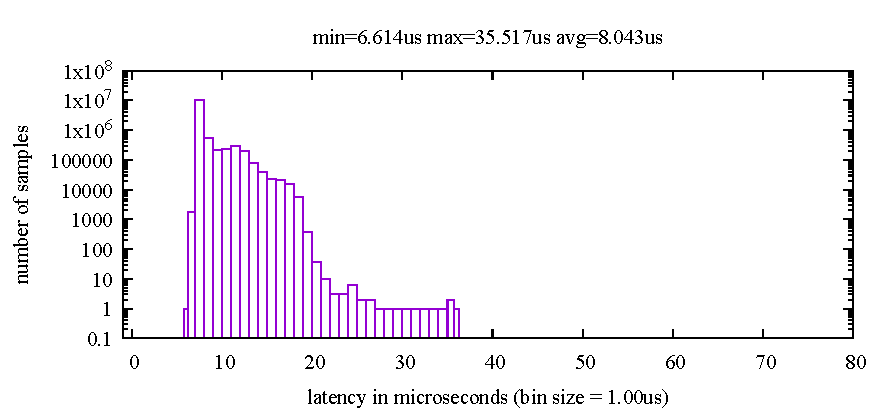
\includegraphics[width=0.45\textwidth]{noworkload-thesis-a}}
        \subfigure[Xenomai]{
            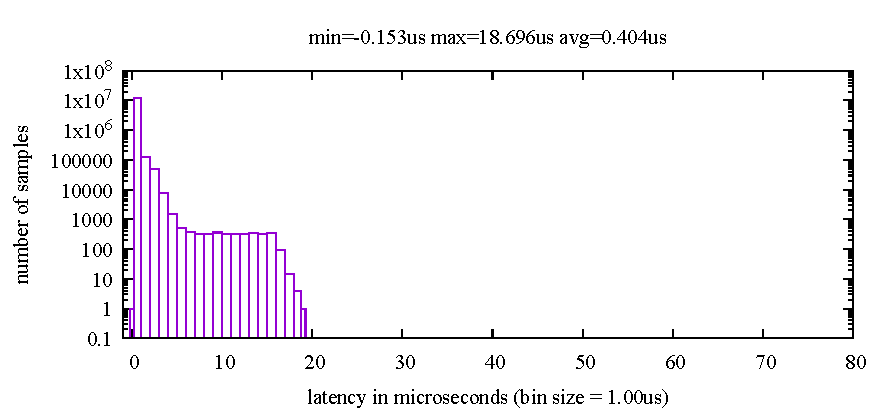
\includegraphics[width=0.45\textwidth]{noworkload-thesis-b}}
    \\
        \subfigure[Xenomai 关闭页迁移]{
            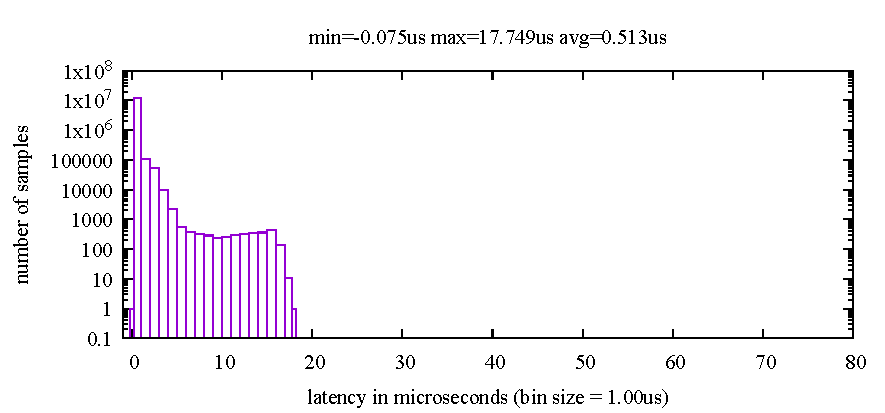
\includegraphics[width=0.45\textwidth]{noworkload-thesis-c}}
        \subfigure[Xenomai 关闭页迁移与高延迟外设并优化关键路径]{
            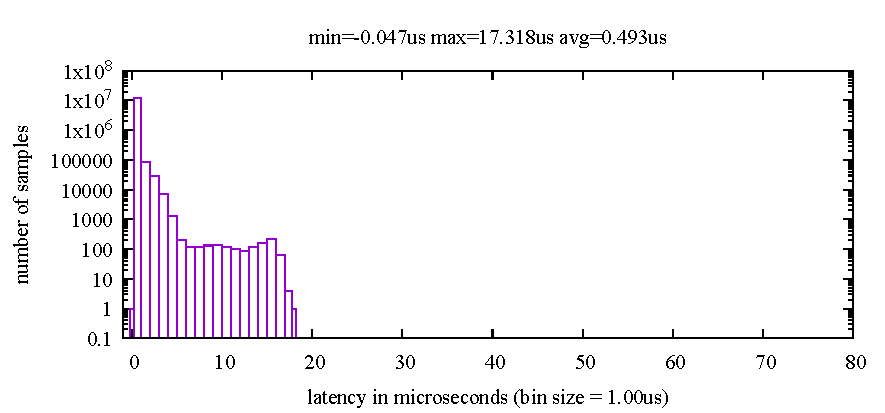
\includegraphics[width=0.45\textwidth]{noworkload-thesis-d}}
    \end{figure}
\end{frame}

\begin{frame}{LoongArch Xenomai 系统的性能优化-访存负载测试结果}
    \begin{figure}[H]
        \centering  %图片全局居中
        \vspace{-0.35cm} %设置与上面正文的距离
        \subfigtopskip=2pt %设置子图与上面正文或别的内容的距离
        \subfigbottomskip=2pt %设置第二行子图与第一行子图的距离,即下面的头与上面的脚的距离
        \subfigcapskip=-5pt %设置子图与子标题之间的距离
        \subfigure[RTLinux]{
            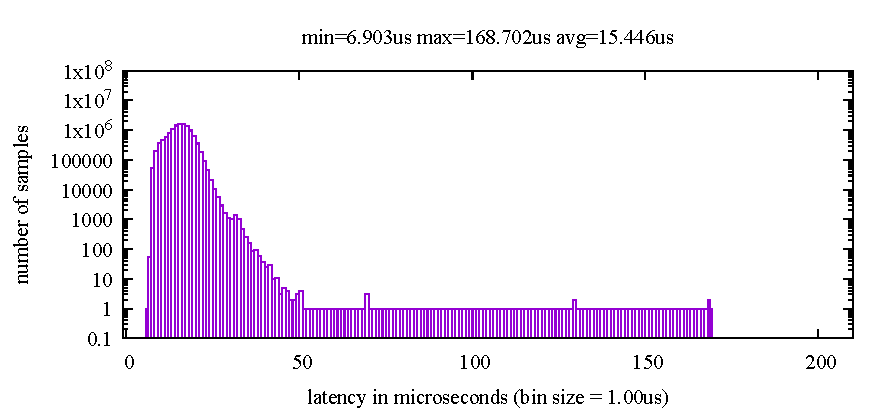
\includegraphics[width=0.45\textwidth]{4vm-thesis-a}}
        \subfigure[Xenomai]{
            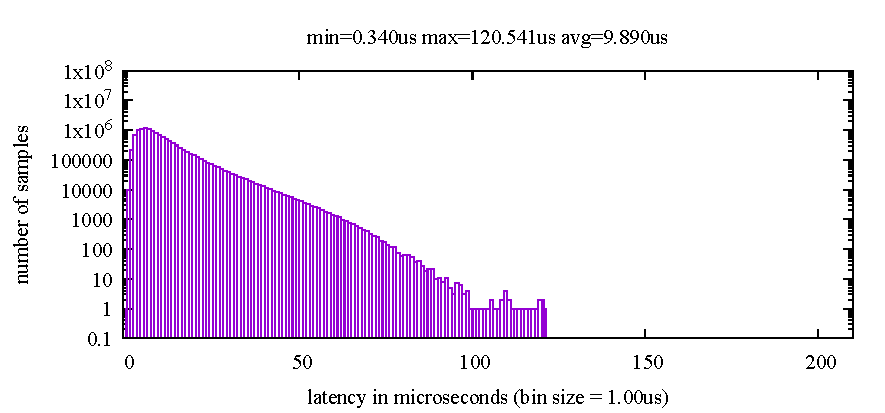
\includegraphics[width=0.45\textwidth]{4vm-thesis-b}}
    \\
        \subfigure[Xenomai 关闭页迁移]{
            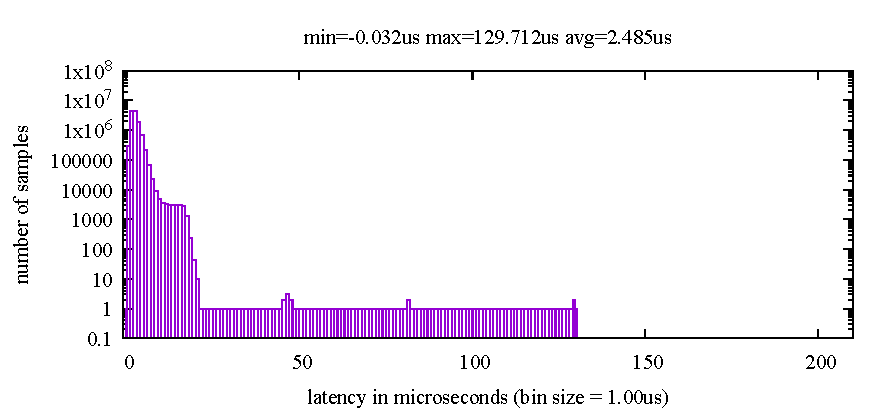
\includegraphics[width=0.45\textwidth]{4vm-thesis-c}}
        \subfigure[Xenomai 关闭页迁移与高延迟外设并优化关键路径]{
            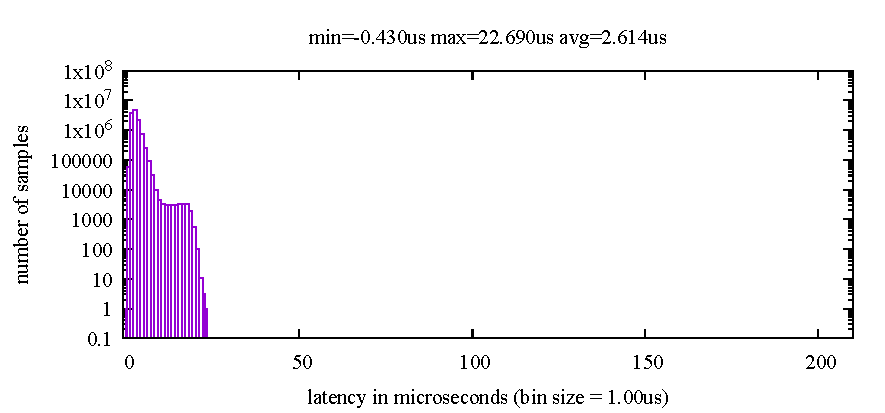
\includegraphics[width=0.45\textwidth]{4vm-thesis-d}}
    \end{figure}
\end{frame}

\begin{frame}{LoongArch Xenomai 系统的性能优化-结论}
    通过关闭页迁移,关闭高延迟外设和关键路径优化,可以使龙芯3A5000+7A2000平台上的Xenomai系统\textbf{达到硬实时要求}
\end{frame}
\section{总结与展望}

\begin{frame}{总结}
    \begin{itemize}
        \item 提出一种由外部事件驱动的\textbf{实时任务模型}
        \item 将Xenomai项目\textbf{移植到LoongArch平台}
        \item 根据LoongArch平台的具体特点,结合实时任务模型进行\textbf{分析优化}
    \end{itemize}
\end{frame}

\begin{frame}{展望}
    \begin{itemize}
        \item \textbf{充分验证。}未来需要对系统进行大量测试以验证移植实现的正确性。
        \item \textbf{嵌入式平台。}未来将Xenomai系统运行在LoongArch嵌入式平台仍需要进一步的移植适配工作。
        \item \textbf{充分优化。}未来需要充分结合LoongArch体系结构与龙芯CPU的特点进行优化。
    \end{itemize}
\end{frame}


% \section{指导}

% \begin{frame}{用Beamer很高大上?}
%     \begin{itemize}[<+-| alert@+>] % 当然,除了alert,手动在里面插 \pause 也行
%         \item 大家都会\LaTeX{},好多学校都有自己的Beamer主题
%         \item 中文支持请选择 Xe\LaTeX{} 编译选项
%         \item Overleaf项目地址位于 \url{},可以直接使用
%         \item Github项目地址位于 \url{https://github.com/peng-yq/UCAS-Beamer-Theme},如果有bug或者feature request可以去里面提issue
%     \end{itemize}
% \end{frame}

% \subsection{研究现状}

% \subsubsection{Beamer主题分类}

% \begin{frame}
%     \begin{itemize}
%         \item 有一些 \LaTeX{} 自带的
%         \item \href{https://www.overleaf.com/latex/templates}{Overleaf}上也有很多
%         \item 本模板修改自
%         \newline
%         \url{https://github.com/tuna/THU-Beamer-Theme}
%         \newline
%         仅换了配色和校徽(其他需求可自行修改样式)
%     \end{itemize}
% \end{frame}


% \subsection{研究内容}

% \subsubsection{美化主题}

% \begin{frame}{THU Beamer Themes}
%     \begin{itemize}
%         \item 顶栏使用一行的导航圈
%         \item 中文采用楷书
%         \item 更多该模板的功能可以参考 \url{https://www.latexstudio.net/archives/4051.html}
%         \item 下面列举出了一些Beamer的用法,部分节选自 \url{https://tuna.moe/event/2018/latex/}
%     \end{itemize}
% \end{frame}

% \subsubsection{如何更好地做Beamer}

% \begin{frame}{Why Beamer}
%     \begin{itemize}
%         \item \LaTeX 广泛用于学术界,期刊会议论文模板
%     \end{itemize}
%     \begin{table}[h]
%         \centering
%         \begin{tabular}{c|c}
%             Microsoft\textsuperscript{\textregistered}  Word & \LaTeX \\
%             \hline
%             文字处理工具 & 专业排版软件 \\
%             容易上手,简单直观 & 容易上手 \\
%             所见即所得 & 所见即所想,所想即所得 \\
%             高级功能不易掌握 & 进阶难,但一般用不到 \\
%             处理长文档需要丰富经验 & 和短文档处理基本无异 \\
%             花费大量时间调格式 & 无需担心格式,专心作者内容 \\
%             公式排版差强人意 & 尤其擅长公式排版 \\
%             二进制格式,兼容性差 & 文本文件,易读、稳定 \\
%             付费商业许可 & 自由免费使用 \\
%         \end{tabular}
%     \end{table}
% \end{frame}

% \begin{frame}{排版举例}
%     \begin{exampleblock}{无编号公式} % 加 * 
%         \begin{equation*}
%             J(\theta) = \mathbb{E}_{\pi_\theta}[G_t] = \sum_{s\in\mathcal{S}} d^\pi (s)V^\pi(s)=\sum_{s\in\mathcal{S}} d^\pi(s)\sum_{a\in\mathcal{A}}\pi_\theta(a|s)Q^\pi(s,a)
%         \end{equation*}
%     \end{exampleblock}
%     \begin{exampleblock}{多行多列公式\footnote{如果公式中有文字出现,请用 $\backslash$mathrm\{\} 或者 $\backslash$text\{\} 包含,不然就会变成 $clip$,在公式里看起来比 $\mathrm{clip}$ 丑非常多。}}
%         % 使用 & 分隔
%         \begin{align}
%             Q_\mathrm{target}&=r+\gamma Q^\pi(s^\prime, \pi_\theta(s^\prime)+\epsilon)\\
%             \epsilon&\sim\mathrm{clip}(\mathcal{N}(0, \sigma), -c, c)\nonumber
%         \end{align}
%     \end{exampleblock}
% \end{frame}

% \begin{frame}
%     \begin{exampleblock}{编号多行公式}
%         % Taken from Mathmode.tex
%         \begin{multline}
%             A=\lim_{n\rightarrow\infty}\Delta x\left(a^{2}+\left(a^{2}+2a\Delta x+\left(\Delta x\right)^{2}\right)\right.\label{eq:reset}\\
%             +\left(a^{2}+2\cdot2a\Delta x+2^{2}\left(\Delta x\right)^{2}\right)\\
%             +\left(a^{2}+2\cdot3a\Delta x+3^{2}\left(\Delta x\right)^{2}\right)\\
%             +\ldots\\
%             \left.+\left(a^{2}+2\cdot(n-1)a\Delta x+(n-1)^{2}\left(\Delta x\right)^{2}\right)\right)\\
%             =\frac{1}{3}\left(b^{3}-a^{3}\right)
%         \end{multline}
%     \end{exampleblock}
% \end{frame}

% \begin{frame}{图形与分栏}
%     \begin{minipage}[c]{0.3\linewidth}
%         \psset{unit=0.8cm}
%         \begin{pspicture}(-1.75,-3)(3.25,4)
%             \psline[linewidth=0.25pt](0,0)(0,4)
%             \rput[tl]{0}(0.2,2){$\vec e_z$}
%             \rput[tr]{0}(-0.9,1.4){$\vec e$}
%             \rput[tl]{0}(2.8,-1.1){$\vec C_{ptm{ext}}$}
%             \rput[br]{0}(-0.3,2.1){$\theta$}
%             \rput{25}(0,0){%
%             \psframe[fillstyle=solid,fillcolor=lightgray,linewidth=.8pt](-0.1,-3.2)(0.1,0)}
%             \rput{25}(0,0){%
%             \psellipse[fillstyle=solid,fillcolor=yellow,linewidth=3pt](0,0)(1.5,0.5)}
%             \rput{25}(0,0){%
%             \psframe[fillstyle=solid,fillcolor=lightgray,linewidth=.8pt](-0.1,0)(0.1,3.2)}
%             \rput{25}(0,0){\psline[linecolor=red,linewidth=1.5pt]{->}(0,0)(0.,2)}
% %           \psRotation{0}(0,3.5){$\dot\phi$}
% %           \psRotation{25}(-1.2,2.6){$\dot\psi$}
%             \psline[linecolor=red,linewidth=1.25pt]{->}(0,0)(0,2)
%             \psline[linecolor=red,linewidth=1.25pt]{->}(0,0)(3,-1)
%             \psline[linecolor=red,linewidth=1.25pt]{->}(0,0)(2.85,-0.95)
%             \psarc{->}{2.1}{90}{112.5}
%             \rput[bl](.1,.01){C}
%         \end{pspicture}
%     \end{minipage}\hspace{1cm}
%     \begin{minipage}{0.5\linewidth}
%         \medskip
%         %\hspace{2cm}
%         \begin{figure}[h]
%             \centering
%             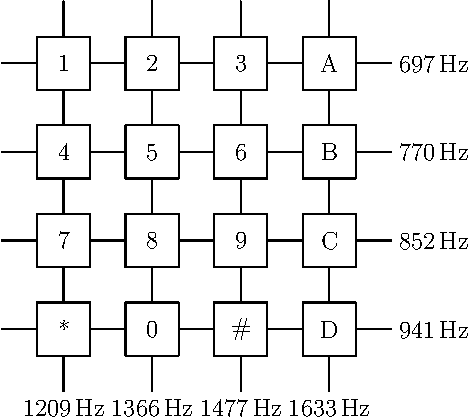
\includegraphics[height=.4\textheight]{pic/dtmf.pdf}
%         \end{figure}
%     \end{minipage}
% \end{frame}

% \begin{frame}[fragile]{\LaTeX{} 常用命令}
%     \begin{exampleblock}{命令}
%         \centering
%         \footnotesize
%         \begin{tabular}{llll}
%             \cmd{chapter} & \cmd{section} & \cmd{subsection} & \cmd{paragraph} \\
%             章 & 节 & 小节 & 带题头段落 \\\hline
%             \cmd{centering} & \cmd{emph} & \cmd{verb} & \cmd{url} \\
%             居中对齐 & 强调 & 原样输出 & 超链接 \\\hline
%             \cmd{footnote} & \cmd{item} & \cmd{caption} & \cmd{includegraphics} \\
%             脚注 & 列表条目 & 标题 & 插入图片 \\\hline
%             \cmd{label} & \cmd{cite} & \cmd{ref} \\
%             标号 & 引用参考文献 & 引用图表公式等\\\hline
%         \end{tabular}
%     \end{exampleblock}
%     \begin{exampleblock}{环境}
%         \centering
%         \footnotesize
%         \begin{tabular}{lll}
%             \env{table} & \env{figure} & \env{equation}\\
%             表格 & 图片 & 公式 \\\hline
%             \env{itemize} & \env{enumerate} & \env{description}\\
%             无编号列表 & 编号列表 & 描述 \\\hline
%         \end{tabular}
%     \end{exampleblock}
% \end{frame}

% \begin{frame}[fragile]{\LaTeX{} 环境命令举例}
%     \begin{minipage}{0.5\linewidth}
% \begin{lstlisting}[language=TeX]
% \begin{itemize}
%   \item A \item B
%   \item C
%   \begin{itemize}
%     \item C-1
%   \end{itemize}
% \end{itemize}
% \end{lstlisting}
%     \end{minipage}\hspace{1cm}
%     \begin{minipage}{0.3\linewidth}
%         \begin{itemize}
%             \item A
%             \item B
%             \item C
%             \begin{itemize}
%                 \item C-1
%             \end{itemize}
%         \end{itemize}
%     \end{minipage}
%     \medskip
%     \pause
%     \begin{minipage}{0.5\linewidth}
% \begin{lstlisting}[language=TeX]
% \begin{enumerate}
%   \item 巨佬 \item 大佬
%   \item 萌新
%   \begin{itemize}
%     \item[n+e] 瑟瑟发抖
%   \end{itemize}
% \end{enumerate}
% \end{lstlisting}
%     \end{minipage}\hspace{1cm}
%     \begin{minipage}{0.3\linewidth}
%         \begin{enumerate}
%             \item 巨佬
%             \item 大佬
%             \item 萌新
%             \begin{itemize}
%                 \item[n+e] 瑟瑟发抖
%             \end{itemize}
%         \end{enumerate}
%     \end{minipage}
% \end{frame}

% \begin{frame}[fragile]{\LaTeX{} 数学公式}
%     \begin{columns}
%         \begin{column}{.55\textwidth}
% \begin{lstlisting}[language=TeX]
% $V = \frac{4}{3}\pi r^3$

% \[
%   V = \frac{4}{3}\pi r^3
% \]

% \begin{equation}
%   \label{eq:vsphere}
%   V = \frac{4}{3}\pi r^3
% \end{equation}
% \end{lstlisting}
%         \end{column}
%         \begin{column}{.4\textwidth}
%             $V = \frac{4}{3}\pi r^3$
%             \[
%                 V = \frac{4}{3}\pi r^3
%             \]
%             \begin{equation}
%                 \label{eq:vsphere}
%                 V = \frac{4}{3}\pi r^3
%             \end{equation}
%         \end{column}
%     \end{columns}
%     \begin{itemize}
%         \item 更多内容请看 \href{https://zh.wikipedia.org/wiki/Help:数学公式}{\color{red}{这里}}
%     \end{itemize}
% \end{frame}

% \begin{frame}[fragile]
%     \begin{columns}
%         \column{.6\textwidth}
% \begin{lstlisting}[language=TeX]
%     \begin{table}[htbp]
%       \caption{编号与含义}
%       \label{tab:number}
%       \centering
%       \begin{tabular}{cl}
%         \toprule
%         编号 & 含义 \\
%         \midrule
%         1 & 4.0 \\
%         2 & 3.7 \\
%         \bottomrule
%       \end{tabular}
%     \end{table}
%     公式~(\ref{eq:vsphere}) 的
%     编号与含义请参见
%     表~\ref{tab:number}。
% \end{lstlisting}
%         \column{.4\textwidth}
%         \begin{table}[htpb]
%             \centering
%             \caption{编号与含义}
%             \label{tab:number}
%             \begin{tabular}{cl}\toprule
%                 编号 & 含义 \\\midrule
%                 1 & 4.0\\
%                 2 & 3.7\\\bottomrule
%             \end{tabular}
%         \end{table}
%         \normalsize 公式~(\ref{eq:vsphere})的编号与含义请参见表~\ref{tab:number}。
%     \end{columns}
% \end{frame}

% \begin{frame}{作图}
%     \begin{itemize}
%         \item 矢量图 eps, ps, pdf
%         \begin{itemize}
%             \item METAPOST, pstricks, pgf $\ldots$
%             \item Xfig, Dia, Visio, Inkscape $\ldots$
%             \item Matlab / Excel 等保存为 pdf
%         \end{itemize}
%         \item 标量图 png, jpg, tiff $\ldots$
%         \begin{itemize}
%             \item 提高清晰度,避免发虚
%             \item 应尽量避免使用
%         \end{itemize}
%     \end{itemize}
% \end{frame}

% \section{参考文献}

% \begin{frame}[allowframebreaks]
%     \bibliography{ref}
%     \tiny\bibliographystyle{ieeetr}
%     \nocite{*}
%     % 如果参考文献太多的话,可以像下面这样调整字体:
%     % \tiny\bibliographystyle{alpha}
% \end{frame}

\begin{frame}
    \begin{center}
        {\Huge 请各位专家老师批评指正!}
    \end{center}
\end{frame}

\end{document}